% paper/part1_main.tex
% Part 1: HoloForge -- Systematic Degradation Analysis in Phase-Only
% Computational Holography (revised version v2, 2026-09-26).
%
% Build:  pdflatex part1_main.tex  (x2 for references). Figures resolve via
%         \graphicspath to ../code/results/.
%
% TRACEABILITY. Every number in this file is copied from a CSV written by
% ../code/run_experiments.py (or ../code/gs_target_fidelity.py), rounded as
% printed. Source per table:
%   Tab. I  (reference scene, all axes) .... results/metrics_summary.csv
%   Tab. II (across five scenes) ........... results/multi_scene_summary.csv
%   Tab. III (per-scene, phase bits) ....... results/multi_scene_metrics.csv
%   Tab. IV (five GS seeds) ................ results/seed_sensitivity_summary.csv
%   Tab. V  (GS vs. target) ................ results/gs_vs_target.csv
%   Spectral energy ........................ results/viewing_energy.csv
%   GS convergence ......................... results/gs_convergence.npy
% Evidence classes: [L] literature/established theory (cited), [P] stated
% simulation parameter, [D] derived here from stated inputs, [S] simulation
% output of this study. Interpretations are labelled as such.

\documentclass[conference]{IEEEtran}
\usepackage{amsmath,amssymb,graphicx,booktabs,hyperref,cite,xcolor}
\usepackage[utf8]{inputenc}
\usepackage[T1]{fontenc}
\graphicspath{{figures/}{../code/results/}}

\title{Systematic Degradation Analysis in Phase-Only\\Computational Holography: A Simulation Framework}

\author{
  \IEEEauthorblockN{Chaitanya Tripathi}
  \IEEEauthorblockA{Ashoka University\\
  Sonipat, India\\
  chaitanya.tripathi\_ug2025@ashoka.edu.in}
}

\begin{document}
\maketitle

\begin{abstract}
We describe \textsc{HoloForge}, an open-source simulation framework that
applies four hardware-motivated degradations -- spatial resolution, phase
quantization, spectral (viewing-angle) bandwidth and random phase noise -- to
Gerchberg--Saxton (GS) phase-only holograms propagated with the angular
spectrum method, and scores each degraded reconstruction against the
undegraded GS reconstruction with PSNR, SSIM and LPIPS. On a low-frequency
reference scene, 4- and 8-bit quantization leave the reconstruction
unchanged to three decimals of SSIM, 2 bits give SSIM $0.978$ and 1 bit
$0.655$. Across five scenes the loss is strongly content-dependent: mean
SSIM is $0.934$ at 4 bits, $0.636$ at 2 bits and $0.273$ at 1 bit, and the
natural photograph falls to $0.255$ at 2 bits. The 1-bit loss is consistent
with the twin image that any real-valued hologram must carry. All results are
simulation outputs, no human observers were involved, and the code and data
reproduce every number in about a minute on a CPU.
\end{abstract}

\begin{IEEEkeywords}
holography, spatial light modulator, phase retrieval, Gerchberg--Saxton,
angular spectrum method, image quality metrics, simulation
\end{IEEEkeywords}

% ----------------------------------------------------------------------
\section{Introduction}
Holographic near-eye displays are a candidate technology for
depth-correct augmented and virtual reality~\cite{maimone2017holographic,shi2021towards}.
Phase-only spatial light modulators (SLMs) are the usual substrate, and their
reconstruction quality is bounded by pixel count, the number of addressable
phase levels, the angular bandwidth of the optics and phase errors of the
device~[L]. These effects are usually studied while proposing a new
method~\cite{choi2022time,peng2020neural,chakravarthula2019wirtinger,shi2021towards}.
This paper does the narrower thing: it holds the scene, propagation model and
retrieval algorithm fixed and varies one degradation at a time, with open
code. We do not claim the effects are new; the contribution is a controlled,
reproducible baseline.

Contributions:
\begin{enumerate}
\item An open simulation framework combining established components -- the
      angular spectrum method (ASM)~\cite{goodman2005introduction} and GS phase
      retrieval~\cite{gerchberg1972practical} [L] -- with four degradation
      operators applied to the complex SLM field before propagation.
\item Simulated measurements of how each degradation changes the
      reconstruction, on one reference scene, across five scenes and across
      five GS initializations [S].
\item An account of the 1-bit quantization loss as the twin image forced on
      any real-valued hologram~\cite{gabor1948new}, derived from the
      quantizer's output levels [D] and checked against the simulations [S].
\end{enumerate}

\textbf{How claims are sourced.} Established theory and literature results
are cited [L]; simulation settings are stated [P]; results derived here from
stated inputs are marked [D]; numbers produced by our simulations are [S].
Every [S] number is copied from a CSV written by the released scripts (see
Code and Data Availability). Interpretations beyond the data are labelled.

% ----------------------------------------------------------------------
\section{Related Work}
\label{sec:related}
\textbf{SLM constraints.} Pixel pitch sets the diffraction angle
($\sin\theta\approx\lambda/2\Delta x$) and, with pixel count, the
space--bandwidth product and \'etendue of a holographic display~\cite{holoeye2023slm}
[L]. Fast, heavily quantized SLMs have been compensated algorithmically by
time-multiplexed neural holography~\cite{choi2022time}. Binary
computer-generated holograms~\cite{brown1966complex,lee1978computer} carry a
conjugate (twin) image~\cite{gabor1948new} [L].

\textbf{Phase retrieval.} GS~\cite{gerchberg1972practical} alternates
amplitude constraints between the hologram and image planes; Fienup's
input--output variants~\cite{fienup1982phase} improve convergence and
stagnation; gradient-based (Wirtinger) holography~\cite{chakravarthula2019wirtinger},
learned models~\cite{shi2021towards} and camera-in-the-loop
optimization~\cite{peng2020neural} reach higher reconstruction quality than GS
[L]. We use GS because it is deterministic given a seed and widely
understood; the degradation thresholds of optimization-based methods may
differ and are not studied here.

\textbf{Image-quality metrics.} PSNR measures pixel error; SSIM~\cite{wang2004image}
combines luminance, contrast and structure; LPIPS~\cite{zhang2018unreasonable}
compares deep-network features and, on the distortion types studied by its
authors, agrees better with human similarity judgements than PSNR or SSIM
[L]. We report all three. None of them has been validated for holographic
artefacts in this work.

% ----------------------------------------------------------------------
\section{Optical Model and Simulation Framework}
\label{sec:method}
\subsection{Propagation: angular spectrum method [L]+[P]}
A monochromatic field $U(x,y,0)$ is propagated by
$U(x,y,z)=\mathcal{F}^{-1}\{\hat U(f_x,f_y)H(f_x,f_y,z)\}$ with
$H=\exp\!\big(j2\pi z\sqrt{\lambda^{-2}-f_x^2-f_y^2}\big)$ for
$f_x^2+f_y^2\le\lambda^{-2}$ and $0$ otherwise~\cite{goodman2005introduction}.
Parameters [P]: $\lambda=532$\,nm, $z=150$\,mm, pixel pitch
$\Delta x=8\,\mu$m, $256\times256$ grid. The implementation conserves energy
to within 1\% and inverts ($+z$ then $-z$) to numerical precision; both are
unit tests [S].

\subsection{Phase retrieval: Gerchberg--Saxton [L]+[P]}
From a random initial phase (seed 42 unless stated), GS alternately imposes
the target amplitude at the image plane and unit amplitude at the SLM
plane~\cite{gerchberg1972practical}, for 50 iterations [P]. On the reference
scene the normalized-amplitude MSE between reconstruction and target falls
from $8.7\times10^{-2}$ after one iteration to $7.5\times10^{-4}$ after 30,
$7.1\times10^{-4}$ after 50 and $6.8\times10^{-4}$ after 100
(Fig.~\ref{fig:gs_convergence}) [S]; we use 50.

\subsection{Degradation operators [P]}
Each operator acts on the retrieved SLM phase before reconstruction.

\textbf{D1 resolution.} The phasor $e^{j\phi}$ (real and imaginary parts, to
avoid phase-wrap artefacts) is downsampled from $256\times256$ to $n\times n$
by nearest-neighbour sampling and upsampled back, $n\in\{128,64,32,16\}$.

\textbf{D2 phase quantization.} $b\in\{8,4,2,1\}$ bits with a mid-rise
quantizer on the phase circle,
$\phi_q=\frac{2\pi}{2^b}\big(\lfloor(\phi+\pi)2^b/2\pi\rfloor+\tfrac12\big)-\pi$,
which gives exactly $2^b$ distinct phasors. At $b=1$ the levels are
$\pm\pi/2$, i.e.\ the phasors $\pm j$ [D].

\textbf{D3 spectral bandwidth.} The phasor's spectrum is masked to a disc of
radius $\beta f_{\max}$, $f_{\max}=1/(2\Delta x)$,
$\beta\in\{0.75,0.5,0.25,0.1\}$, and the phase of the masked field is kept.
Because the disc is inscribed in the square Nyquist band, even $\beta=1$
removes spectral energy (on average $0.80$ of it is retained) [S]. We call
this axis ``viewing-angle bandwidth'' because the retained spatial
frequencies set the diffraction angles.

\textbf{D4 phase noise.} Zero-mean Gaussian phase noise of standard deviation
$\sigma\in\{0.1,0.3,0.6,1.0,\pi\}$\,rad is added to the SLM phase before
propagation, modelling SLM phase error and surface roughness; its intensity
effect (speckle) arises through propagation. One noise realization
(seed 0) is used per $\sigma$.

Colour (multi-wavelength) and multi-plane holography are out of scope; the
code keeps a complex-field multi-plane superposition routine as a
demonstration only.

\subsection{Metrics and reference convention}
We compute PSNR, SSIM~\cite{wang2004image} and LPIPS (AlexNet
backbone)~\cite{zhang2018unreasonable} on normalized intensities.
\textbf{All degradation metrics compare a degraded reconstruction with the
undegraded GS reconstruction of the same scene, not with the target.} They
therefore isolate the loss caused by the degradation and exclude GS's own
error; ``SSIM $=1.000$'' means ``indistinguishable from the undegraded GS
output at three decimals'', not ``identical to the target''. For context,
Table~\ref{tab:gstarget} reports the undegraded GS reconstruction against each
target [S]: it ranges from SSIM $0.990$ (reference scene) to $0.505$
(resolution chart).

% ----------------------------------------------------------------------
\section{Experimental Protocol}
\label{sec:experiments}
\textbf{Scenes [P].} (1) \textit{gaussian\_spots}, four Gaussian blobs, the
low-frequency reference scene; (2) \textit{resolution\_chart}, bar gratings
with periods 4--64 px; (3) \textit{letters}, ``HOLO''; (4)
\textit{circle\_ring}, concentric rings; (5) \textit{natural\_photo}, the
scikit-image ``cameraman'' photograph.

\textbf{Statistics [P].} All four axes are run on the reference scene. D1--D3
are repeated on all five scenes (mean $\pm$ standard deviation across scenes;
the spread reflects content, not sampling noise). D1 and D2 are repeated on the
reference scene with five GS seeds $\{42,7,123,999,17\}$ (mean $\pm$ standard
deviation across seeds). Five scenes and five seeds are small samples; we
report spreads, not confidence intervals.

\textbf{Reproducibility.} Ten unit tests check physical invariants (ASM
energy and invertibility, GS convergence, reconstruction range, quantizer
level counts, complex-field superposition, phase-noise range, metric sanity)
and pass. \texttt{python run\_experiments.py} regenerates every result in about
one minute on a laptop CPU; rerunning it reproduces the committed CSVs to
within $10^{-6}$ (LPIPS varies in the seventh decimal).

% ----------------------------------------------------------------------
\section{Results}
\label{sec:results}
All numbers in this section are simulation outputs [S].

\begin{table}[t]
\centering
\caption{Undegraded GS reconstruction vs.\ target (context for the
reconstruction-referenced metrics). \texttt{gs\_vs\_target.csv}.}
\label{tab:gstarget}
\begin{tabular}{lccc}
\toprule
Scene & PSNR (dB) & SSIM & LPIPS \\
\midrule
\textit{gaussian\_spots} & $44.45$ & $0.990$ & $0.057$ \\
\textit{letters} & $23.81$ & $0.899$ & $0.041$ \\
\textit{circle\_ring} & $18.61$ & $0.710$ & $0.083$ \\
\textit{natural\_photo} & $23.78$ & $0.709$ & $0.213$ \\
\textit{resolution\_chart} & $10.47$ & $0.505$ & $0.381$ \\
\bottomrule
\end{tabular}
\end{table}

\begin{figure}[t]
\centering
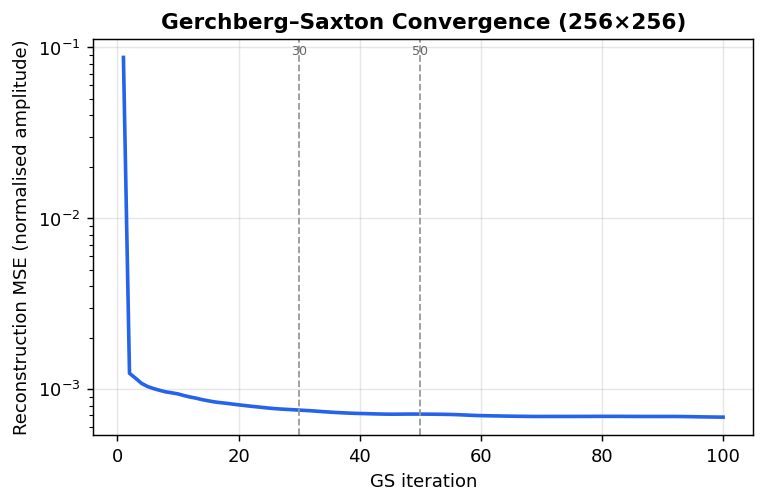
\includegraphics[width=\columnwidth]{gs_convergence.png}
\caption{GS convergence on the reference scene: normalized-amplitude MSE vs.\
target over 100 iterations [S]. Dashed lines: 30 and 50 iterations.}
\label{fig:gs_convergence}
\end{figure}

\subsection{D1: Spatial resolution}
\begin{figure}[t]
\centering
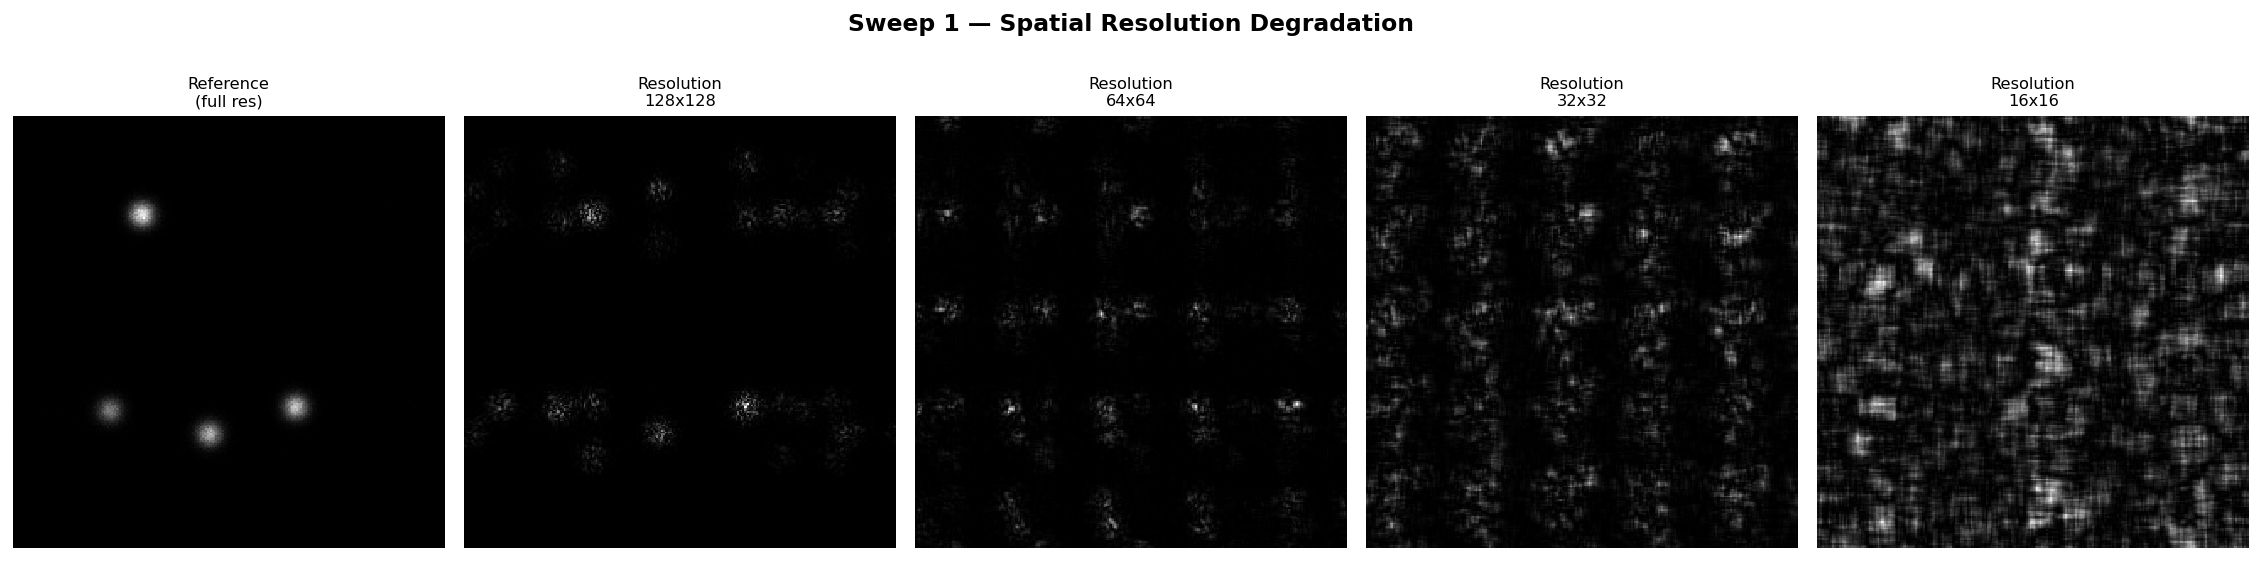
\includegraphics[width=\columnwidth]{sweep_resolution.png}
\caption{Reference-scene reconstructions at effective SLM resolutions 256
(undegraded), 128, 64, 32 and 16 [S].}
\label{fig:resolution}
\end{figure}
\begin{table}[t]
\centering
\caption{Resolution sweep, mean $\pm$ std across five scenes [S].}
\label{tab:resolution}
\begin{tabular}{lccc}
\toprule
Resolution & PSNR (dB) & SSIM & LPIPS \\
\midrule
128$\times$128 & $17.03 \pm 6.69$ & $0.388 \pm 0.313$ & $0.659 \pm 0.220$ \\
64$\times$64   & $15.99 \pm 5.74$ & $0.228 \pm 0.231$ & $0.705 \pm 0.085$ \\
32$\times$32   & $14.66 \pm 4.03$ & $0.085 \pm 0.072$ & $0.757 \pm 0.045$ \\
16$\times$16   & $13.05 \pm 2.22$ & $0.052 \pm 0.020$ & $0.837 \pm 0.075$ \\
\bottomrule
\end{tabular}
\end{table}
All three across-scene means worsen monotonically as resolution falls
(Table~\ref{tab:resolution}). On the reference scene the decline is gradual
(SSIM $0.860$ at 128, $0.657$ at 64); the large across-scene spread comes from
scenes with fine detail (resolution chart, photograph), which lose structure
at the first downsampling step.

\subsection{D2: Phase quantization}
\begin{figure}[t]
\centering
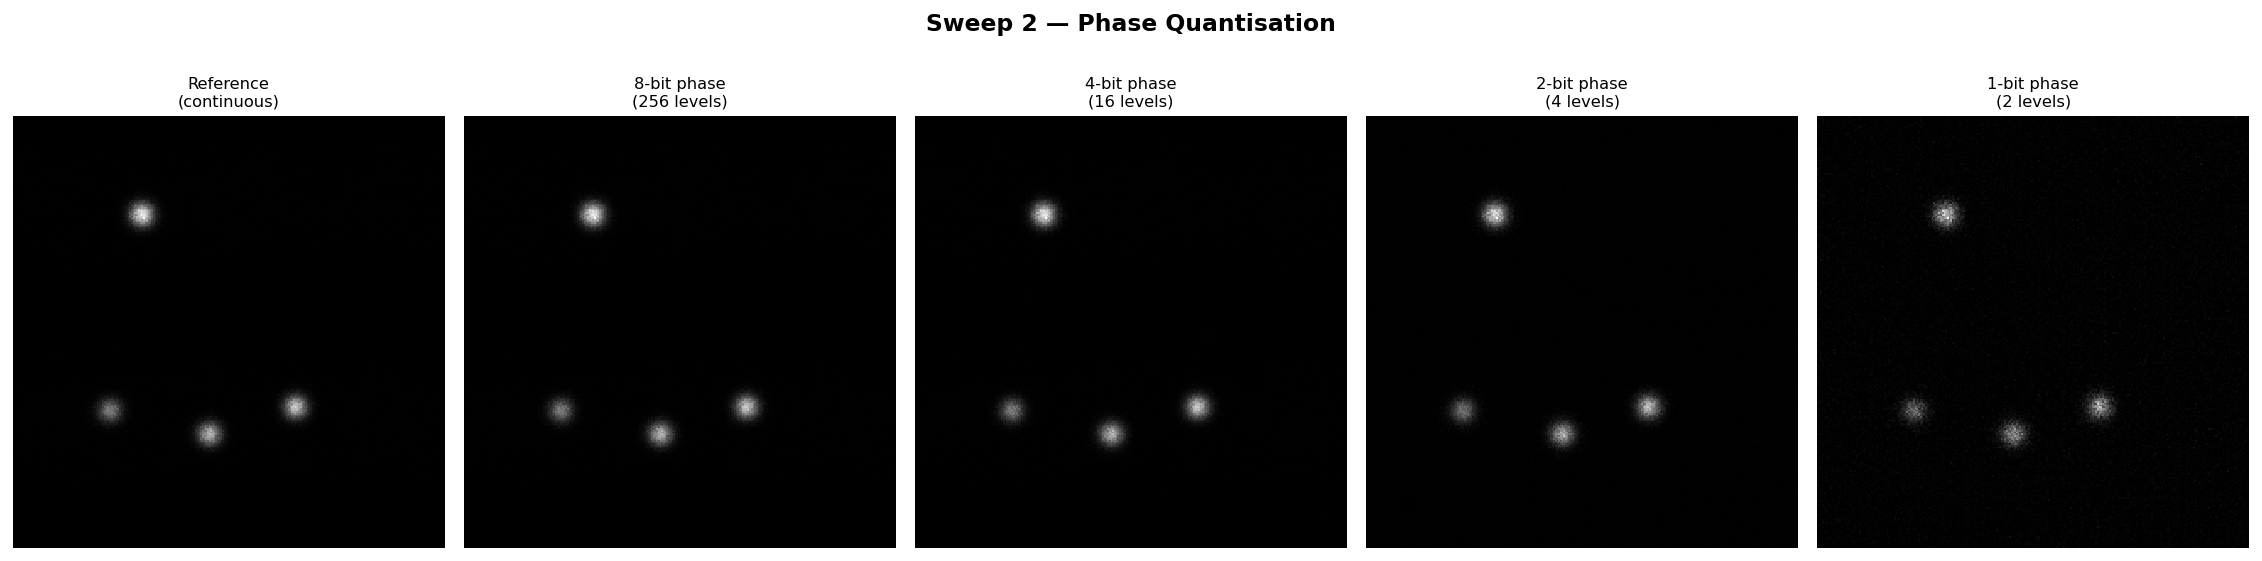
\includegraphics[width=\columnwidth]{sweep_phase_bits.png}
\caption{Reference-scene reconstructions at 8, 4, 2 and 1 bit [S].}
\label{fig:phase_bits}
\end{figure}
\begin{table}[t]
\centering
\caption{All four axes on the reference scene [S]
(\texttt{metrics\_summary.csv}).}
\label{tab:phase_bits}
\begin{tabular}{llccc}
\toprule
Axis & Setting & PSNR (dB) & SSIM & LPIPS \\
\midrule
Bits & 8 & $83.0$ & $1.000$ & $0.000$ \\
     & 4 & $59.4$ & $1.000$ & $0.000$ \\
     & 2 & $45.0$ & $0.978$ & $0.016$ \\
     & 1 & $35.7$ & $0.655$ & $0.180$ \\
\midrule
Bandwidth & 75\% & $31.1$ & $0.978$ & $0.171$ \\
          & 50\% & $28.9$ & $0.968$ & $0.164$ \\
          & 25\% & $29.7$ & $0.972$ & $0.108$ \\
          & 10\% & $29.2$ & $0.728$ & $0.148$ \\
\midrule
Noise $\sigma$ & 0.1 & $60.1$ & $1.000$ & $0.000$ \\
     & 0.3 & $49.7$ & $0.994$ & $0.005$ \\
     & 0.6 & $42.7$ & $0.915$ & $0.053$ \\
     & 1.0 & $34.9$ & $0.501$ & $0.258$ \\
     & $\pi$ & $18.5$ & $0.008$ & $0.963$ \\
\bottomrule
\end{tabular}
\end{table}
On the reference scene, 8- and 4-bit quantization leave the reconstruction
unchanged at three decimals of SSIM, 2 bits give $0.978$ and 1 bit $0.655$
(Table~\ref{tab:phase_bits}). The reference scene is the most tolerant of the
five, however (Table~\ref{tab:perscene}): at 4 bits the natural photograph
already falls to $0.749$, and at 2 bits the across-scene mean is
$0.636\pm0.250$, with the photograph at $0.255$. At 1 bit the across-scene
mean is $0.273\pm0.198$. Across five GS seeds on the reference scene the
1-bit SSIM is $0.600\pm0.028$ (Table~\ref{tab:seed}), so on this scene the
1-bit loss depends little on initialization.

\begin{table}[t]
\centering
\caption{Per-scene SSIM for phase quantization [S]
(\texttt{multi\_scene\_metrics.csv}).}
\label{tab:perscene}
\begin{tabular}{lcccc}
\toprule
Scene & 8-bit & 4-bit & 2-bit & 1-bit \\
\midrule
\textit{gaussian\_spots}   & $1.000$ & $1.000$ & $0.978$ & $0.655$ \\
\textit{letters}           & $1.000$ & $0.997$ & $0.818$ & $0.241$ \\
\textit{circle\_ring}      & $1.000$ & $0.978$ & $0.626$ & $0.213$ \\
\textit{resolution\_chart} & $1.000$ & $0.947$ & $0.504$ & $0.165$ \\
\textit{natural\_photo}    & $0.998$ & $0.749$ & $0.255$ & $0.089$ \\
\midrule
mean $\pm$ std & $1.000\pm0.001$ & $0.934\pm0.095$ & $0.636\pm0.250$ & $0.273\pm0.198$ \\
\bottomrule
\end{tabular}
\end{table}

\subsection{D3: Spectral (viewing-angle) bandwidth}
\begin{figure}[t]
\centering
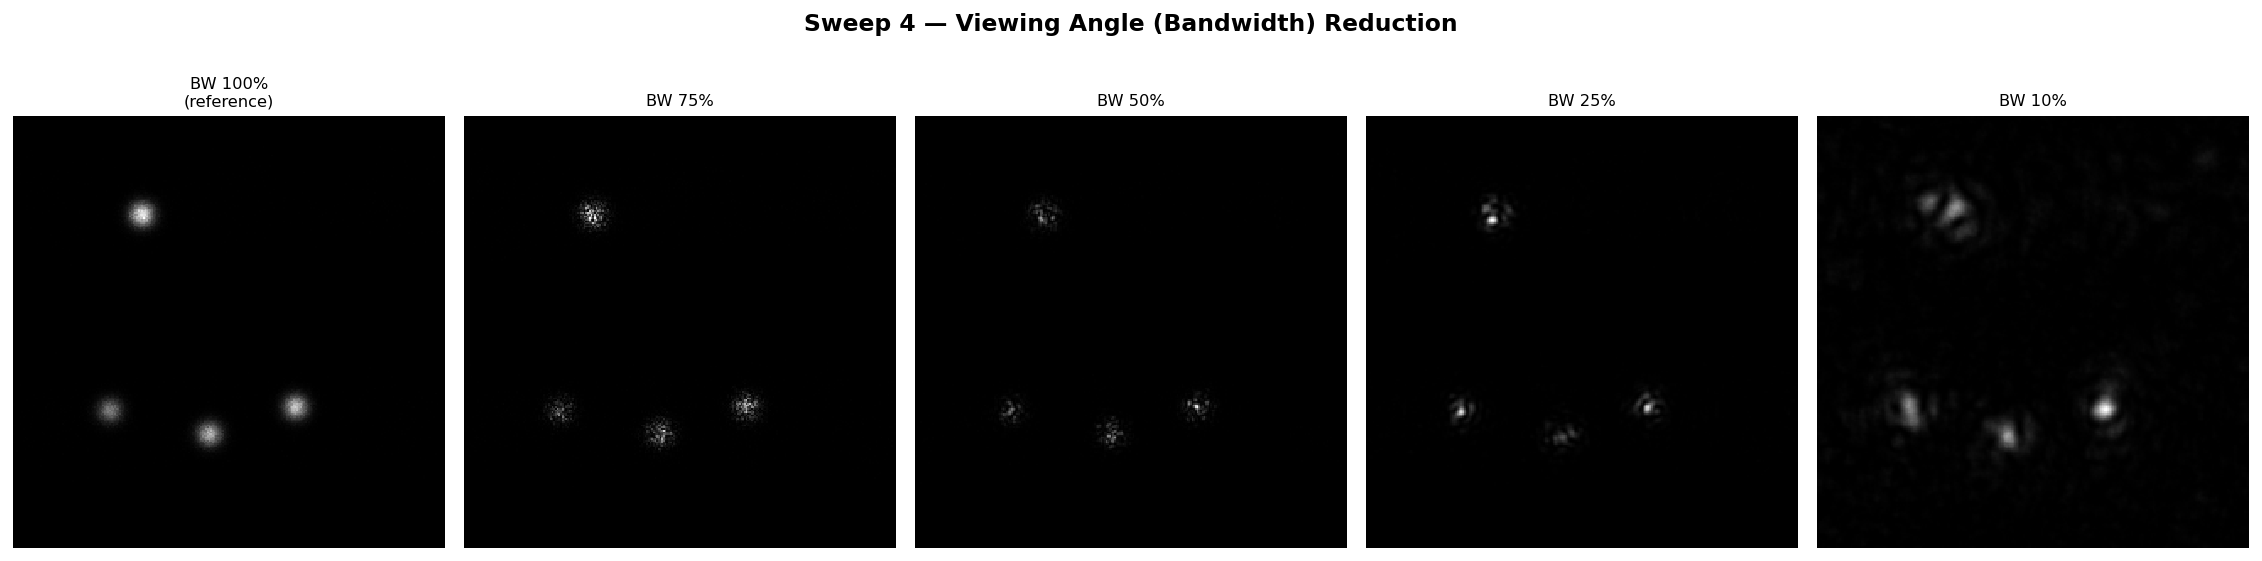
\includegraphics[width=\columnwidth]{sweep_viewing_angle.png}
\caption{Reference-scene reconstructions with the spectrum masked to 75, 50,
25 and 10\% of the Nyquist radius [S].}
\label{fig:viewing_angle}
\end{figure}
\begin{table}[t]
\centering
\caption{Bandwidth sweep, mean $\pm$ std across five scenes [S].}
\label{tab:viewing}
\begin{tabular}{lccc}
\toprule
Bandwidth & PSNR (dB) & SSIM & LPIPS \\
\midrule
75\% & $18.37 \pm 7.28$ & $0.634 \pm 0.293$ & $0.402 \pm 0.232$ \\
50\% & $17.46 \pm 6.72$ & $0.615 \pm 0.297$ & $0.420 \pm 0.244$ \\
25\% & $17.47 \pm 7.02$ & $0.595 \pm 0.306$ & $0.435 \pm 0.257$ \\
10\% & $17.44 \pm 6.66$ & $0.362 \pm 0.202$ & $0.540 \pm 0.221$ \\
\bottomrule
\end{tabular}
\end{table}
On the reference scene SSIM is $0.978$, $0.968$ and $0.972$ at 75, 50 and 25\%
and $0.728$ at 10\%. The across-scene mean falls slowly to 25\% and then
sharply (Table~\ref{tab:viewing}).

The mask is active at every step (Fig.~\ref{fig:viewing_energy}): the
retained fraction of spectral energy averages $0.80$, $0.46$, $0.21$, $0.055$
and $0.008$ at 100, 75, 50, 25 and 10\%. \textbf{Interpretation:} SSIM stays
flat while $\sim$95\% of the spectral energy is removed because, for compact
low-frequency targets, the energy-bearing low-frequency core lies inside the
25\% disc; the drop at 10\% coincides with the mask cutting into that core.
The average hides two behaviours: flat-then-drop for low-frequency scenes
(\textit{gaussian\_spots} $0.978\to0.972$ from 75 to 25\%, then $0.728$), and
low, slowly declining SSIM for broadband ones (\textit{natural\_photo}
$0.237$, $0.218$, $0.163$ at 75, 25, 10\%).

\begin{figure}[t]
\centering
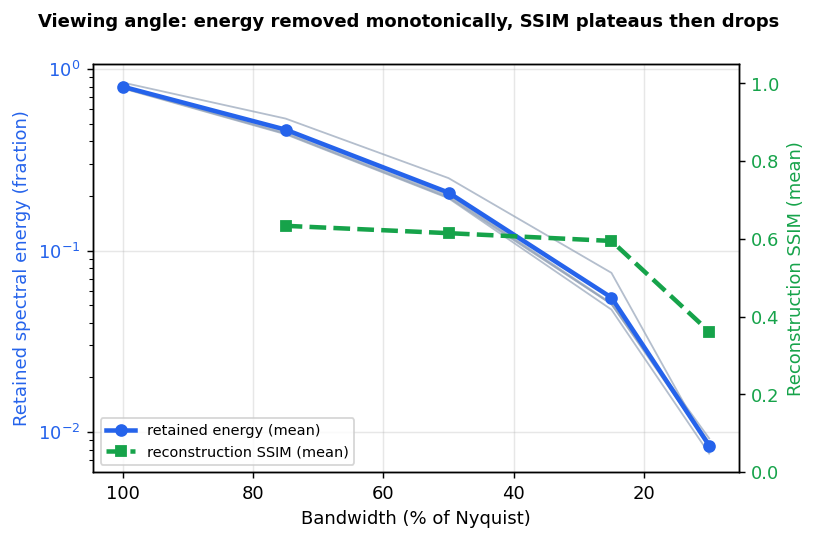
\includegraphics[width=\columnwidth]{viewing_energy.png}
\caption{Retained spectral energy (blue, log axis; grey per scene, thick
mean) and mean reconstruction SSIM (green) vs.\ bandwidth [S].}
\label{fig:viewing_energy}
\end{figure}

\subsection{D4: Phase noise}
\begin{figure}[t]
\centering
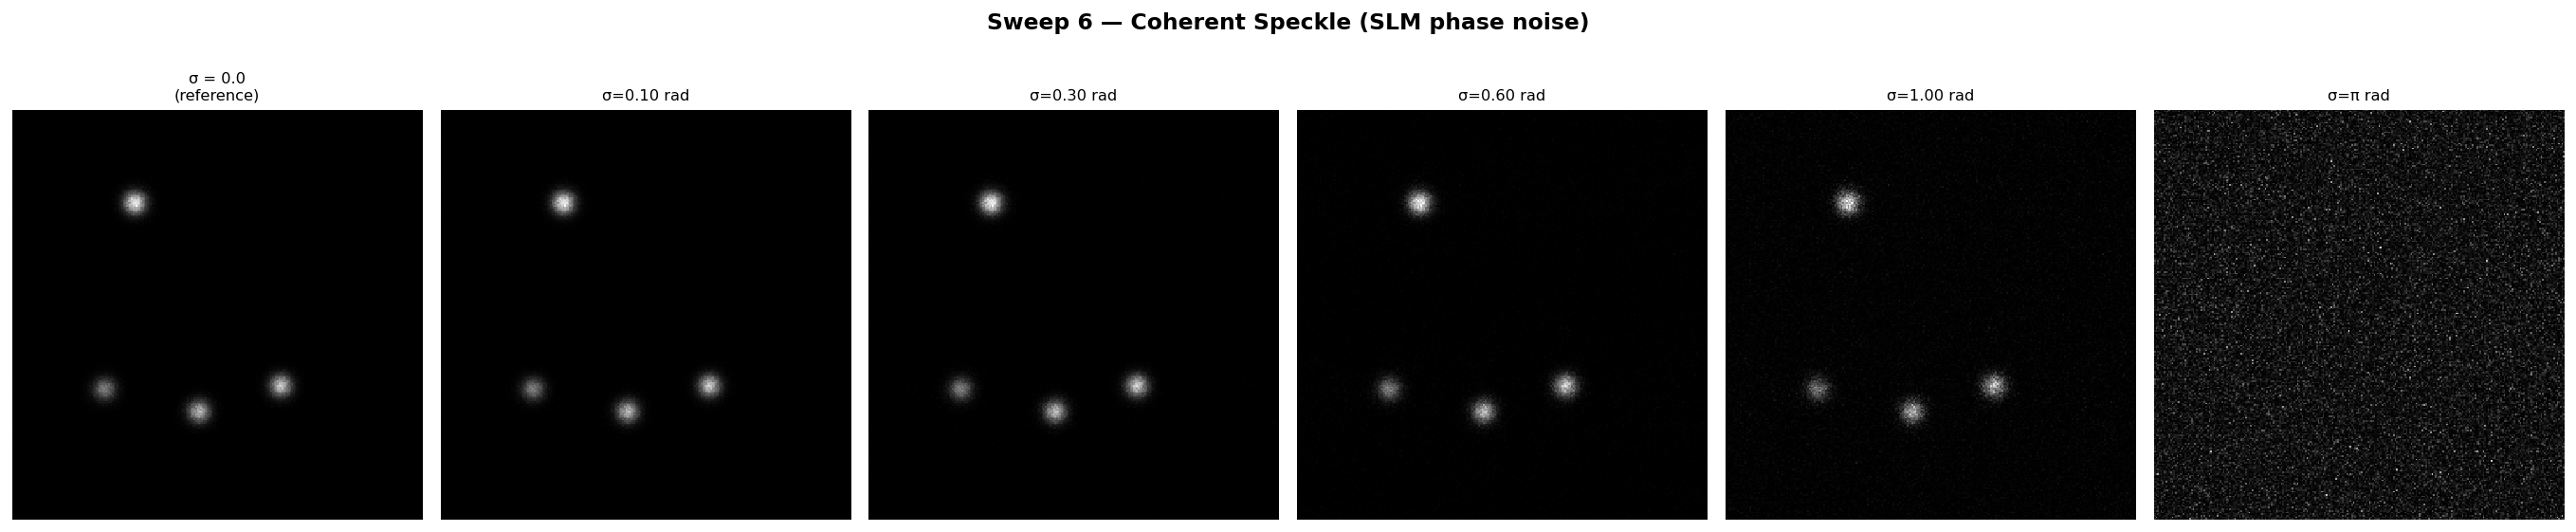
\includegraphics[width=\columnwidth]{sweep_speckle.png}
\caption{Reference-scene reconstructions with aperture-plane phase noise of
increasing $\sigma$ (one realization each) [S].}
\label{fig:speckle}
\end{figure}
On the reference scene (Table~\ref{tab:phase_bits}) SSIM is $\ge0.99$ for
$\sigma\le0.3$\,rad, $0.915$ at $0.6$, $0.501$ at $1.0$ and $0.008$ at $\pi$.
These values come from one noise realization per $\sigma$ on one scene, so they
indicate where the transition lies for this configuration rather than a
general tolerance specification.

\subsection{Agreement between metrics}
\begin{figure}[t]
\centering
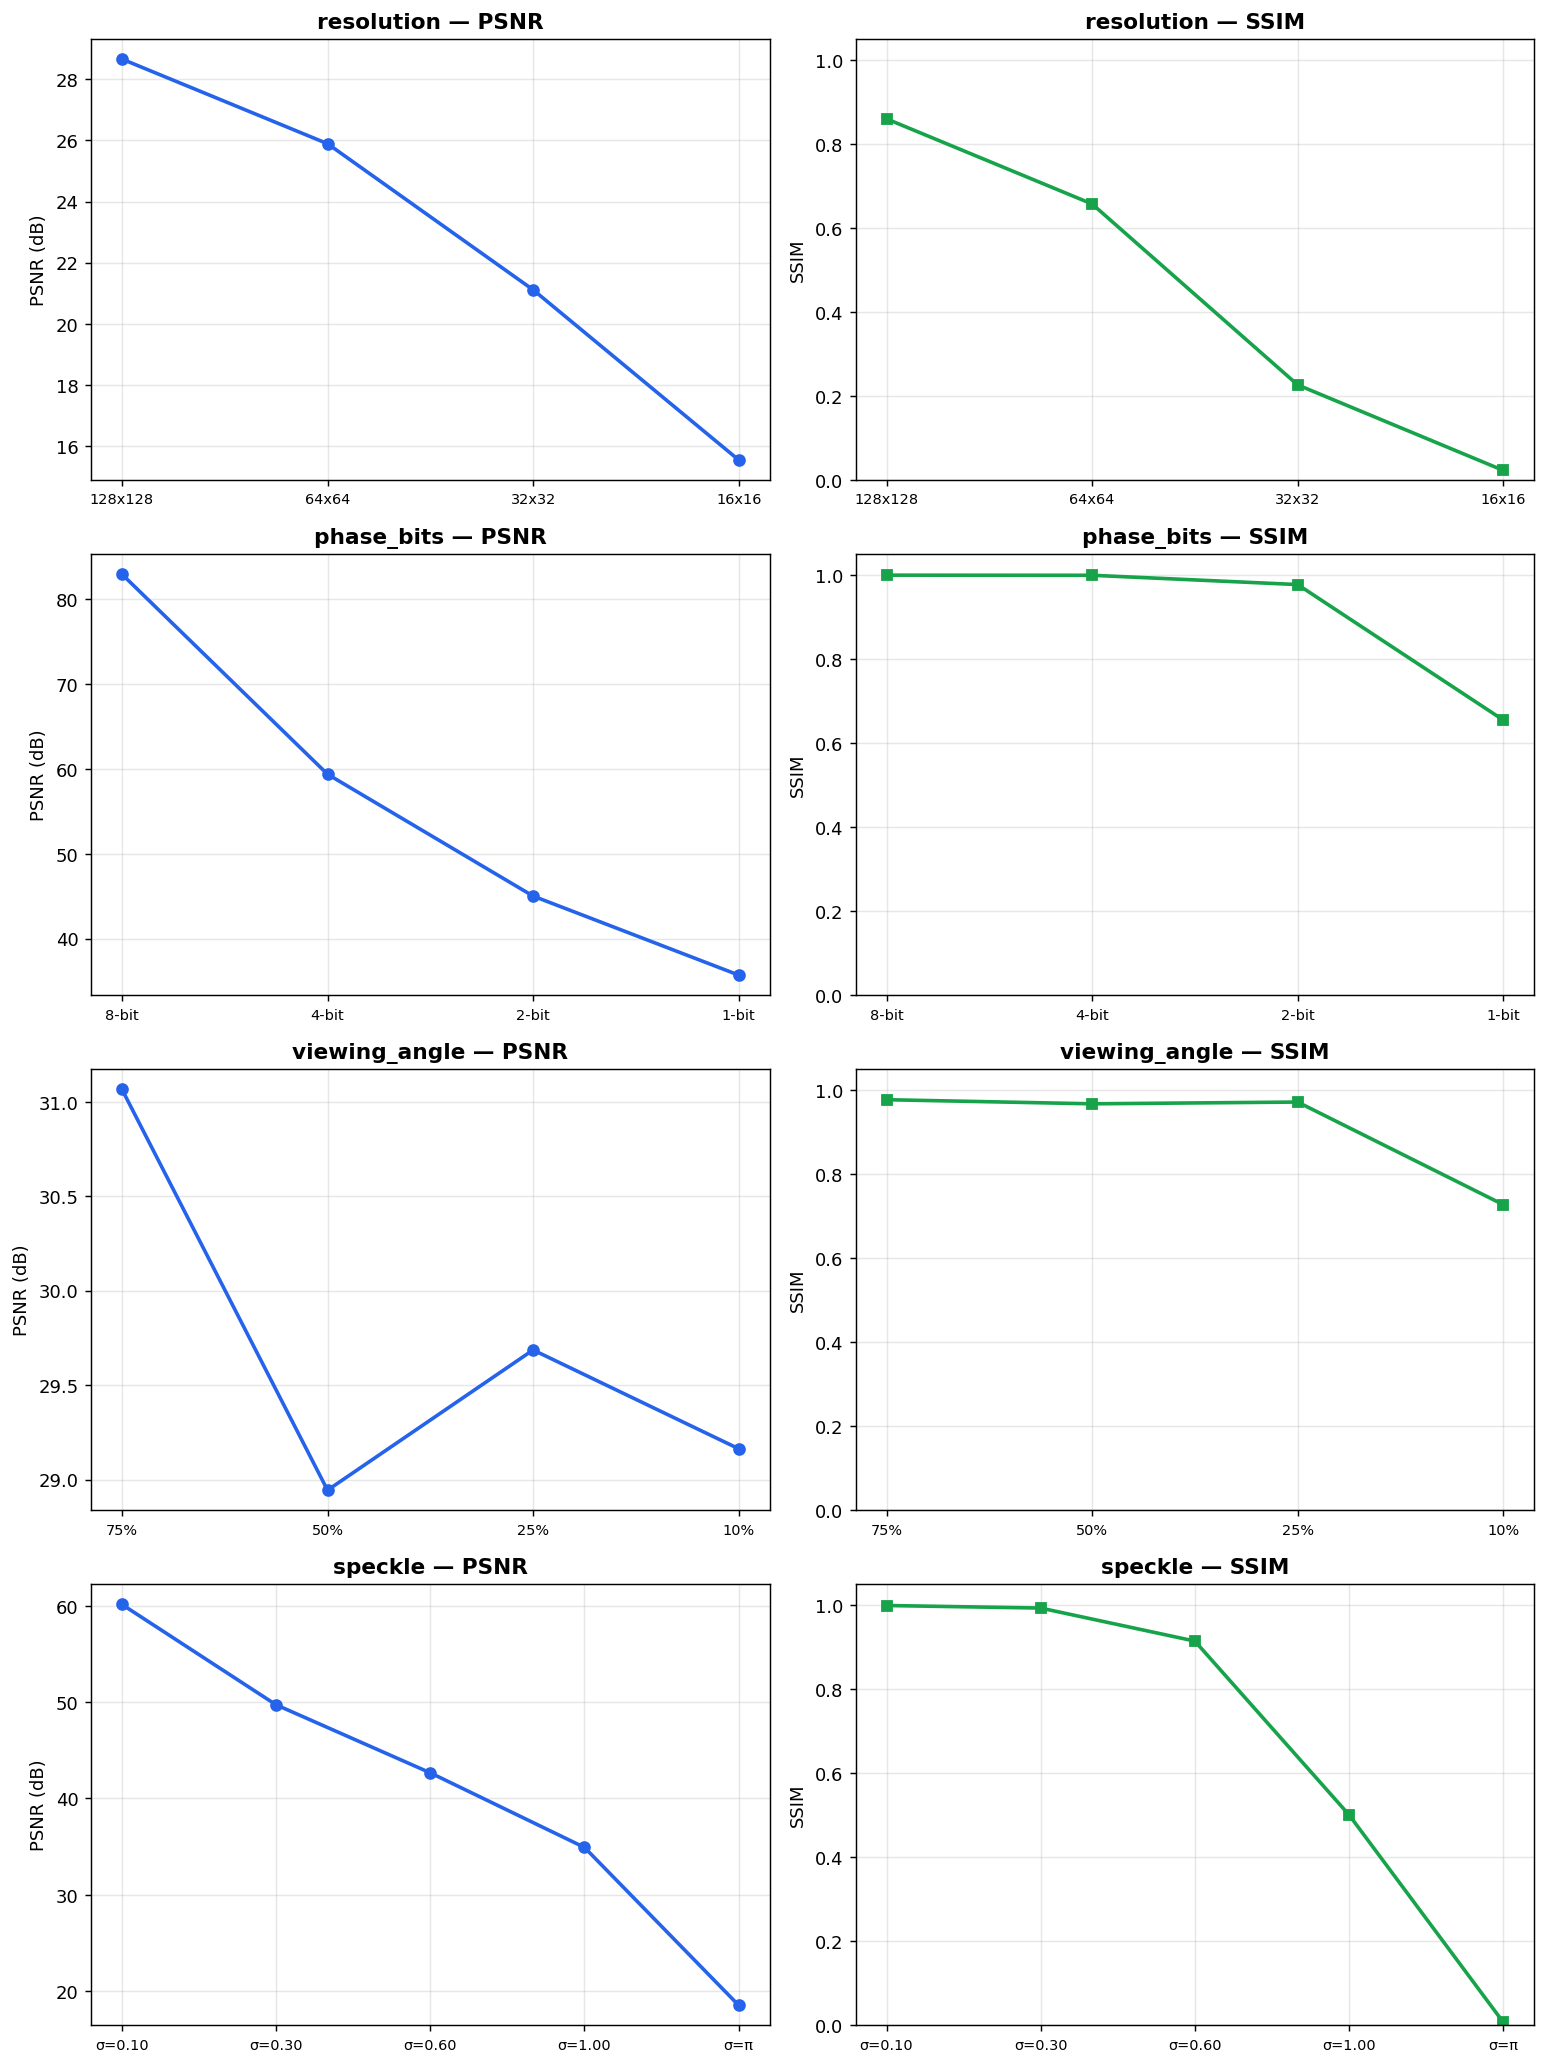
\includegraphics[width=\columnwidth]{metrics_summary_plot.png}
\caption{PSNR and SSIM across the four axes on the reference scene [S].}
\label{fig:metrics_summary}
\end{figure}
\begin{figure}[t]
\centering
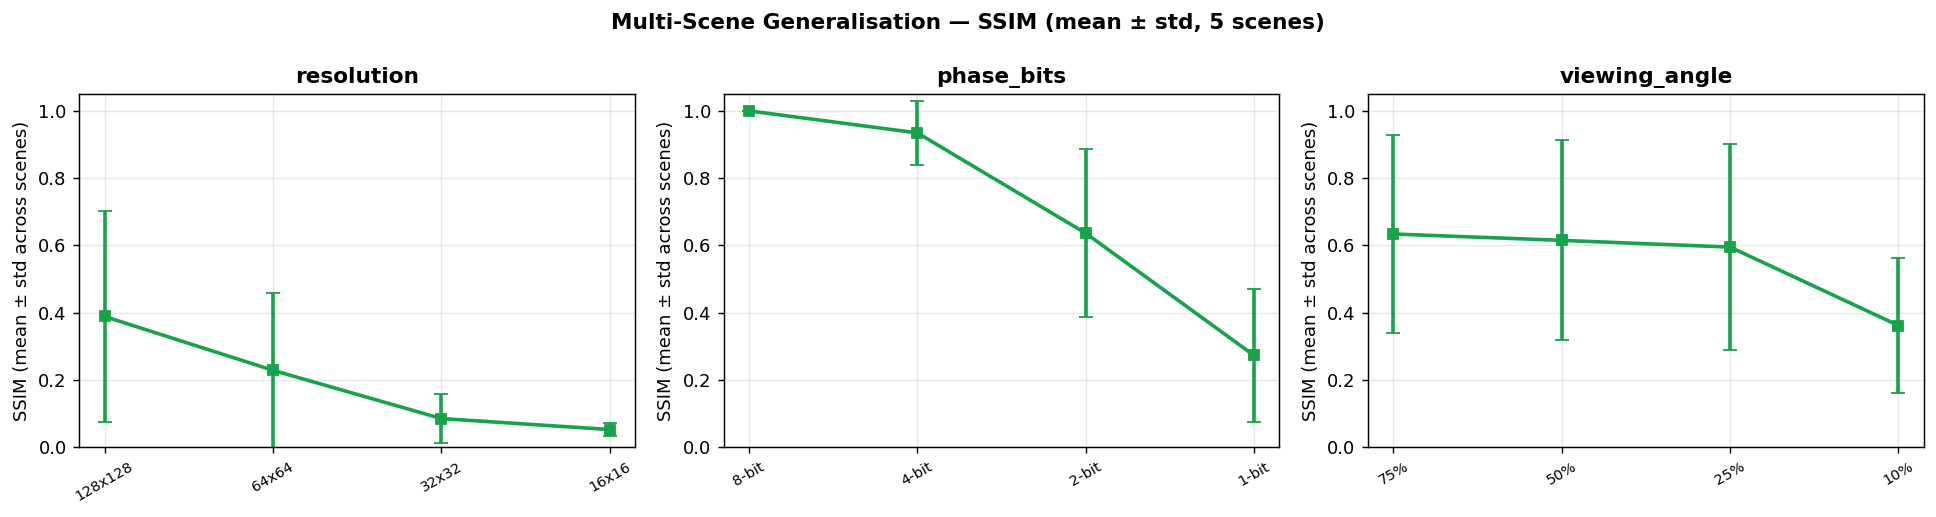
\includegraphics[width=\columnwidth]{multi_scene_summary.png}
\caption{SSIM, mean $\pm$ std across five scenes, for D1--D3 [S].}
\label{fig:multiscene}
\end{figure}
The metrics do not always agree. Under resolution loss (across scenes,
Table~\ref{tab:resolution}) PSNR falls by $4.0$\,dB from 128 to 16 pixels
while SSIM falls from $0.388$ to $0.052$, i.e.\ to about one seventh. In the
reference-scene bandwidth sweep (Table~\ref{tab:phase_bits}) the three
metrics order the settings differently: PSNR ranks 75\% $>$ 25\% $>$ 10\% $>$
50\%, SSIM ranks 75\% $>$ 25\% $>$ 50\% $>$ 10\%, and LPIPS ranks 25\% best and
75\% worst. Which metric better predicts what an observer
would see is not tested here.

\begin{table}[t]
\centering
\caption{Five GS seeds, reference scene, mean $\pm$ std [S]
(\texttt{seed\_sensitivity\_summary.csv}).}
\label{tab:seed}
\begin{tabular}{llccc}
\toprule
Sweep & Setting & PSNR (dB) & SSIM & LPIPS \\
\midrule
Bits & 8 & $82.93 \pm 0.70$ & $1.000 \pm 0.000$ & $0.000 \pm 0.000$ \\
Bits & 4 & $59.23 \pm 0.22$ & $1.000 \pm 0.000$ & $0.000 \pm 0.000$ \\
Bits & 2 & $45.66 \pm 0.79$ & $0.975 \pm 0.002$ & $0.019 \pm 0.004$ \\
Bits & 1 & $35.93 \pm 0.22$ & $0.600 \pm 0.028$ & $0.202 \pm 0.011$ \\
Res. & 128 & $28.63 \pm 0.24$ & $0.860 \pm 0.009$ & $0.381 \pm 0.017$ \\
Res. & 64  & $25.55 \pm 0.59$ & $0.627 \pm 0.034$ & $0.583 \pm 0.022$ \\
Res. & 32  & $21.27 \pm 1.08$ & $0.239 \pm 0.031$ & $0.781 \pm 0.026$ \\
Res. & 16  & $17.23 \pm 1.09$ & $0.036 \pm 0.010$ & $0.895 \pm 0.021$ \\
\bottomrule
\end{tabular}
\end{table}
Across GS seeds the standard deviations are at most $1.09$\,dB (PSNR) and
$0.034$ (SSIM) (Table~\ref{tab:seed}), small compared with the differences
between settings; across scenes they are much larger, so content, not
initialization, dominates the variability in these simulations.

% ----------------------------------------------------------------------
\section{Discussion}
\label{sec:discussion}
\subsection{The 1-bit loss and the twin image}
\textbf{Established [L].} A real-valued transmittance cannot distinguish a
field from its complex conjugate, so its reconstruction contains the target
together with a conjugate (twin) term~\cite{gabor1948new}. For the ASM
transfer function, $H(-z)=H(z)^*$, so for real input the fields propagated
to $+z$ and $-z$ are complex conjugates of each other.

\textbf{Derived [D].} The 1-bit mid-rise quantizer outputs the phasors
$\pm j$, i.e.\ $j$ times a real $\pm1$ pattern. A 1-bit hologram is therefore
real-valued up to a global phase, and every hologram GS could output under
this constraint carries the twin term; for $b\ge2$ the output is complex and
the twin is not forced. The argument predicts a qualitative change at 1 bit;
it does not predict the size of the loss, nor that 2 bits will be nearly
lossless.

\textbf{Observed [S].} The 1-bit loss appears in all five scenes and all five
seeds, the reconstruction keeps coarse structure (reference SSIM $0.655$), and
the seed spread is small ($0.028$), which is consistent with a deterministic,
encoding-induced artefact. We did not isolate the twin term directly (for
example by imaging the $-z$ plane), so the attribution is an explanation
consistent with the data rather than a separate measurement.

\subsection{Interpretation for hardware choices}
\textbf{Interpretation.} For GS holography of compact, low-frequency targets
like the reference scene, 2 phase bits would lose little (SSIM $0.978$) and 4
bits nothing measurable. That does not generalize to broadband content: the
natural photograph reaches only $0.749$ at 4 bits and $0.255$ at 2 bits,
relative to its own undegraded reconstruction. Bit-depth requirements
therefore depend on scene content, and these simulations do not support a
content-independent threshold. Similarly, the flat region of the bandwidth
sweep suggests that low-frequency content tolerates a narrow spectral
aperture, while broadband content does not. These readings rest on one
algorithm, one geometry and five scenes.

\subsection{Limitations}
\textit{No human observers.} All quality statements are metric values; this
study makes no claim about perceived quality or perceptual thresholds.
\textit{Reference convention.} Metrics are relative to the undegraded GS
reconstruction, whose own fidelity to the target varies from SSIM $0.99$ to
$0.51$ across scenes (Table~\ref{tab:gstarget}).
\textit{Single algorithm and geometry.} Only GS at one wavelength, distance
and pixel pitch; gradient-based and learned
methods~\cite{chakravarthula2019wirtinger,shi2021towards,peng2020neural} may
respond differently.
\textit{Small samples.} Five scenes (four synthetic), five seeds, and one
noise realization per $\sigma$.
\textit{Idealized device.} No SLM fringing-field, pixel crosstalk, or
nonlinear phase response is modelled.

% ----------------------------------------------------------------------
\section{Conclusion}
\label{sec:conclusion}
\textsc{HoloForge} applies four degradations to GS phase-only holograms in a
controlled, reproducible way. In these simulations the 1-bit quantization
loss is consistent with the twin image forced on real-valued holograms, the
tolerance to reduced bit depth and bandwidth depends strongly on scene
content, and PSNR, SSIM and LPIPS can disagree on the ordering of degradation
settings. Useful next steps are a comparison with gradient-based phase
retrieval under the same degradations and a human-observer study to test
which metric tracks perceived quality. A companion study~\cite{tripathi2026mil}
addresses a different problem, exposure design for write-once photopolymer
media.

\section*{Version note}
This version (v2) corrects the first preprint. v1 described 4-bit quantization
as ``perceptually lossless'' and 2 bits as sufficient ``for these targets'';
both hold only for the reference scene, and no perceptual data were collected.
v1 did not state that metrics are relative to the undegraded GS
reconstruction. v1 said reference-scene SSIM stays above $0.97$ down to 25\%
bandwidth (it is $0.968$ at 50\%). v1 cited speckle $\sigma=1.0$ vs.\ $\pi$ as
a case where SSIM saturates and LPIPS still discriminates (SSIM is $0.501$ vs.\
$0.008$ there, not saturated). v1 announced a human-observer study as Part 2;
Part 2 addresses a different problem. The simulation results are unchanged.

\section*{Code and Data Availability}
Code, unit tests, result CSVs and figures:
\url{https://github.com/ultramagnus23/HoloForge} (\texttt{part1/code/}).
\texttt{python run\_experiments.py} regenerates all results except
Table~\ref{tab:gstarget}, which \texttt{python gs\_target\_fidelity.py}
produces.

\begin{thebibliography}{99}

\bibitem{maimone2017holographic}
A. Maimone, A. Georgiou, and J. S. Kollin, ``Holographic near-eye displays for
virtual and augmented reality,'' \textit{ACM Trans. Graph.}, vol.~36, no.~4,
pp.~1--16, 2017.

\bibitem{shi2021towards}
L. Shi, B. Li, C. Kim, P. Kellnhofer, and W. Matusik, ``Towards real-time
photorealistic 3D holography with deep neural networks,'' \textit{Nature},
vol.~591, pp.~234--239, 2021.

\bibitem{chakravarthula2019wirtinger}
P. Chakravarthula, Y. Peng, J. Kollin, H. Fuchs, and F. Heide, ``Wirtinger
holography for near-eye displays,'' \textit{ACM Trans. Graph.}, vol.~38, no.~6,
pp.~1--13, 2019.

\bibitem{peng2020neural}
Y. Peng, S. Choi, N. Padmanaban, and G. Wetzstein, ``Neural holography with
camera-in-the-loop training,'' \textit{ACM Trans. Graph.}, vol.~39, no.~6,
pp.~1--14, 2020.

\bibitem{choi2022time}
S. Choi, M. Gopakumar, Y. Peng, J. Kim, M. O'Toole, and G. Wetzstein,
``Time-multiplexed neural holography: a flexible framework for holographic
near-eye displays with fast heavily-quantized spatial light modulators,'' in
\textit{ACM SIGGRAPH 2022 Conf. Proc.}, 2022, pp.~1--9.

\bibitem{gerchberg1972practical}
R. W. Gerchberg and W. O. Saxton, ``A practical algorithm for the determination
of phase from image and diffraction plane pictures,'' \textit{Optik}, vol.~35,
pp.~237--246, 1972.

\bibitem{fienup1982phase}
J. R. Fienup, ``Phase retrieval algorithms: a comparison,'' \textit{Appl. Opt.},
vol.~21, no.~15, pp.~2758--2769, 1982.

\bibitem{gabor1948new}
D. Gabor, ``A new microscopic principle,'' \textit{Nature}, vol.~161,
pp.~777--778, 1948.

\bibitem{brown1966complex}
B. R. Brown and A. W. Lohmann, ``Complex spatial filtering with binary masks,''
\textit{Appl. Opt.}, vol.~5, no.~6, pp.~967--969, 1966.

\bibitem{lee1978computer}
W.-H. Lee, ``Computer-generated holograms: techniques and applications,''
\textit{Prog. Opt.}, vol.~16, pp.~119--232, 1978.

\bibitem{goodman2005introduction}
J. W. Goodman, \textit{Introduction to Fourier Optics}, 3rd ed. Englewood,
CO: Roberts and Company, 2005.

\bibitem{holoeye2023slm}
HOLOEYE Photonics AG, ``Spatial light modulators (LCoS phase),'' product
documentation, 2023. [Online]. Available: \url{https://holoeye.com/spatial-light-modulators/}

\bibitem{wang2004image}
Z. Wang, A. C. Bovik, H. R. Sheikh, and E. P. Simoncelli, ``Image quality
assessment: from error visibility to structural similarity,''
\textit{IEEE Trans. Image Process.}, vol.~13, no.~4, pp.~600--612, 2004.

\bibitem{zhang2018unreasonable}
R. Zhang, P. Isola, A. A. Efros, E. Shechtman, and O. Wang, ``The unreasonable
effectiveness of deep features as a perceptual metric,'' in
\textit{Proc. IEEE CVPR}, 2018, pp.~586--595.

\bibitem{tripathi2026mil}
C. Tripathi, ``Media-in-the-loop holography: computer-generated holography
through a differentiable model of volume photopolymer recording,'' manuscript
in preparation, 2026.

\end{thebibliography}

\end{document}
